\scanpage{12}
\mspage{\unsure{6}}
Programme du \deleted{paradigme \unsure{de théorie des|de la théorie des}} \inserted{``gruppentheoretisches} Gleichnis'' (paradigme en termes de théorie des groupes) de l'\inserted{arithmétique :}\deleted{\unsure{arithm.} géométrie algébrique absolue (en car. 0).}

a) Donner une description ``gruppentheoretisch'' complète de $\Gamma$

b) Donner une description complète de tous les éléments de structure énumérés ci-dessus, dans des cas typiques importants pour $(\mathfrak X,D,J)$, dont nous indiquons quelques-uns plus bas.

\margin{On tâchera de prendre $\mathfrak X$ propre autant que possible (quitte à compléter\ldots)}

\uline{NB} Quand on a les éléments de structure envisagés pour $(\mathfrak X,D,J)$, on les a aussi automatiquement pour \unsure{tt|$\forall$} 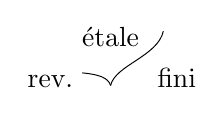
\begin{tikzpicture}[baseline=(rev012.base)]
\node[anchor=base west,inner sep=0pt] (rev012) at (0,0) {rev.};
\node[anchor=base west,inner sep=0pt] at (1.65,0) {fini};
\node[anchor=base,inner sep=0pt] at (1.06,.52) {\inserted{étale}};
\draw[line width=.35pt] (.70,.19) .. controls (.91,.17) and (1.03,.13) .. (1.06,.03);
\draw[line width=.35pt] (1.06,.03) .. controls (1.12,.29) and (1.66,.40) .. (1.73,.72);
\end{tikzpicture} de $\mathfrak X'....$ Il faudrait expliciter ce point avec soin, et expliciter également dans les $=$ optiques les foncteurs ``bouchage de trous'' (en rajoutant 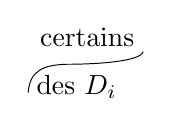
\begin{tikzpicture}[baseline=(des012.base)]
\node[anchor=base west,inner sep=0pt] (des012) at (.12,0) {des $D_i$};
\node[anchor=base,inner sep=0pt] at (.77,.61) {\inserted{certains}};
\draw[line width=.35pt] (.02,.02) .. controls (.04,.31) and (.23,.37) .. (.50,.38)
  .. controls (.93,.38) and (1.45,.42) .. (1.48,.54);
\end{tikzpicture} qu'on avait enlevés) ou ``forage des trous'' 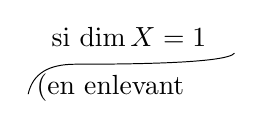
\begin{tikzpicture}[baseline=(en012.base)]
\node[anchor=base west,inner sep=0pt] (en012) at (.12,0) {(en enlevant};
\node[anchor=base,inner sep=0pt] at (1.30,.61) {\inserted{si $\dim\mathfrak X=1$}};
\draw[line width=.35pt] (.02,.01) .. controls (.08,.28) and (.29,.39) .. (.62,.39)
  .. controls (1.28,.39) and (2.54,.40) .. (2.64,.53);
\end{tikzpicture} certains des $\xi\in J$).
\mspage{11}
